\documentclass[11pt,leqno]{article}
\usepackage[margin=1in]{geometry}
\usepackage{graphicx}
\usepackage{amsmath, amsthm, amssymb, latexsym}
\usepackage{enumerate}
\usepackage{color}
\usepackage{hyperref}

\usepackage{url}


\usepackage{float}
% for better float placement, allows "H" ("HERE") as specification 
% for float placement, e.g. 
% \begin{figure}[H]

\graphicspath{{Graphics/}}

%%%%%%%%%%%%%%%%%%%%%%%%%%%%%%%

% theorem declarations

\newtheorem{defn}{Definition}[section]
\newtheorem{thm}[defn]{Theorem}

%%%%%%%%%%%%%%%%%%%%%%%%%%%%%%%


\begin{document}




\title{
Interactive Visualizations in Mathematica 
\\
Final Report, Spring 2021}
\author{Faculty Mentor: A.J. Hildebrand \\
    Project Leader: Efstathios Konstantinos Chrontsios Garitsis \\
	IGL Scholars: Xiaojun Jia, Adithya Swaminathan, \\
	Dimitrios Tambakos, Troy Yang, Sarah Zimmerman}
	\date{May 12, 2021}
\maketitle
\section{Introduction}
This project is part of a long-term
program aimed at creating interactive Mathematica-based visualizations of
interesting mathematical topics and making these available to a broader
audience through publication at the Wolfram Demonstrations website \cite{WD}.
The ultimate goal is to develop a collection of attractive
interactive tools for use in instruction and outreach activities. 

This semester we focused on visualizations of Julia sets 
and of fractals defined in terms of digital sums. 


\section{Julia Sets}
Let $P: \mathbb{C} \rightarrow \mathbb{C}$ be a complex polynomial and 
let $P^k$ denote the $k$-th iterate of $P$,
i.e., $P^k = P \circ \dots \circ P$  $k$-times.

\begin{defn}
The \textbf{Julia set} of $P$ is the boundary of the set of points $z \in
\mathbb{C}$ for which the set $\{P^{k}(z) : k \in \mathbb{N}\}$ is
bounded.  The complement of the Julia set is the \textbf{Fatou set} of $P$.
\end{defn}


Julia sets of \emph{quadratic} polynomials of the form ${z^2 + c}$ have
been extensively studied and many visualizations of such Julia sets have
been created; see, for example, the books by Beardon \cite{beardon} and
Carleson and Gamelin \cite{carleson-gamelin} for an introduction to Complex Dynamics and the relevant visualizations in \cite{WD}. 

In our project, we focused on Julia sets of \emph{cubic}
polynomials.  We are specifically interested in the nature of the Julia
set graph of polynomials of the form 
\begin{equation}
\label{eq:polynomial}
P(z)=z^3+re^{ti}z^2+e^{2 \pi i \theta}z
\end{equation}
as the variables $r>0,\, t\in \mathbb{R},\, \theta \in
\mathbb{R}\setminus\mathbb{Q}$ vary. 

We noticed several symmetry patterns in these graphs.  One such pattern
is illustrated in \mbox{Figure \ref{fig:rotational-symmetry}}: When $r=4$,
$\theta=\pi$ and $t$ varies over the interval $[0,2\pi]$, the
corresponding Julia set graph rotates about the origin by an angle $t$.

\begin{figure}[H]
\label{fig:rotational-symmetry}
\centering
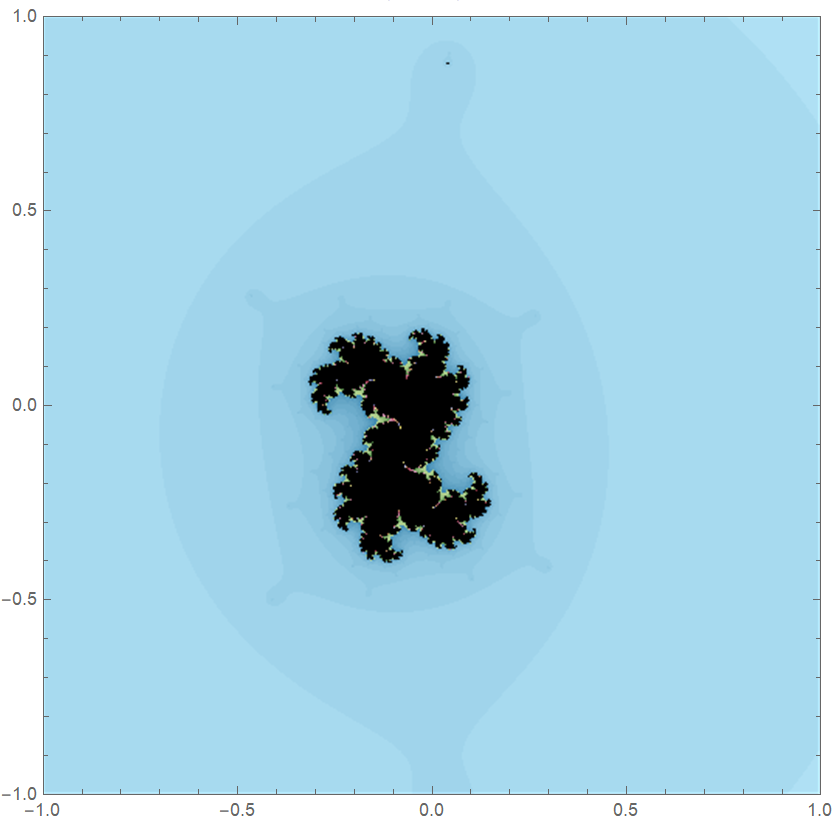
\includegraphics[width=0.4\textwidth,height=0.3\textwidth]{1.PNG}
\hspace{1em}
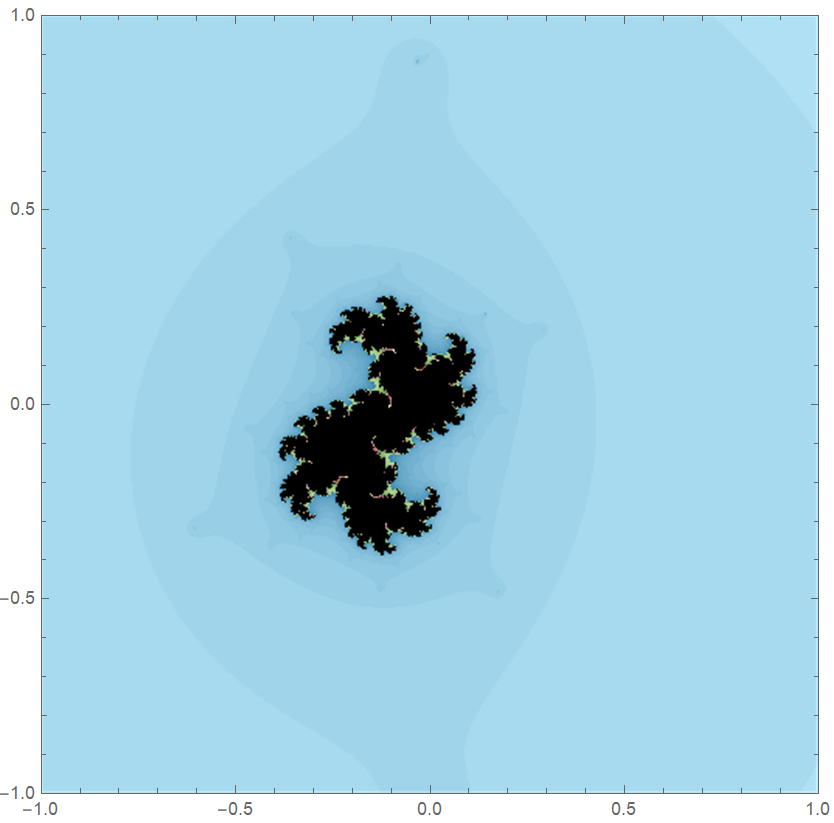
\includegraphics[width=0.4\textwidth,height=0.3\textwidth]{2.PNG}
\\
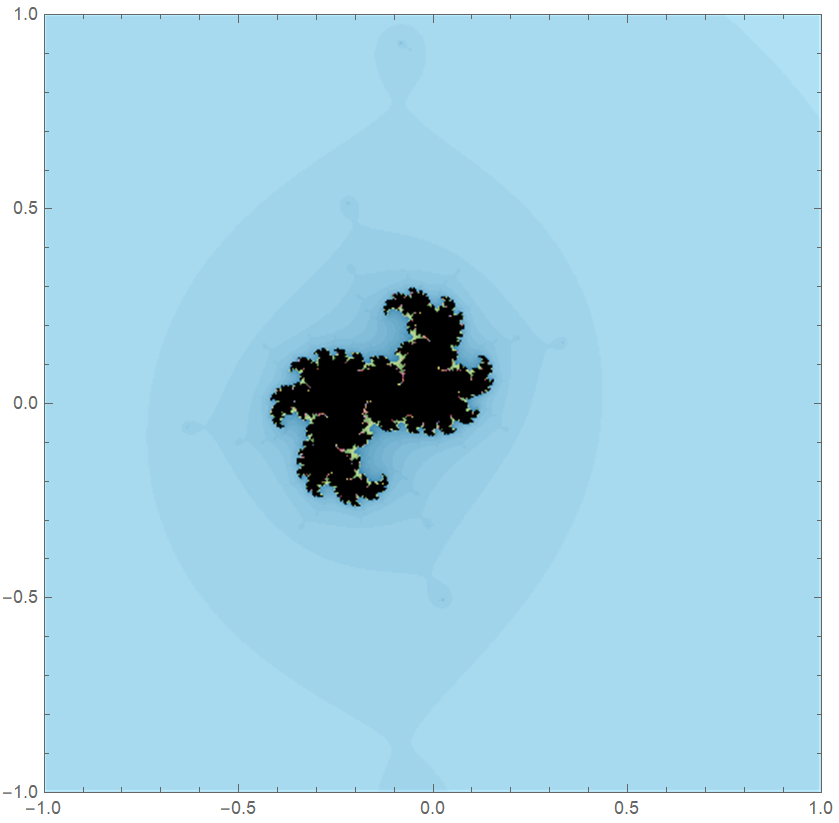
\includegraphics[width=0.4\textwidth,height=0.3\textwidth]{3.PNG}
\hspace{1em}
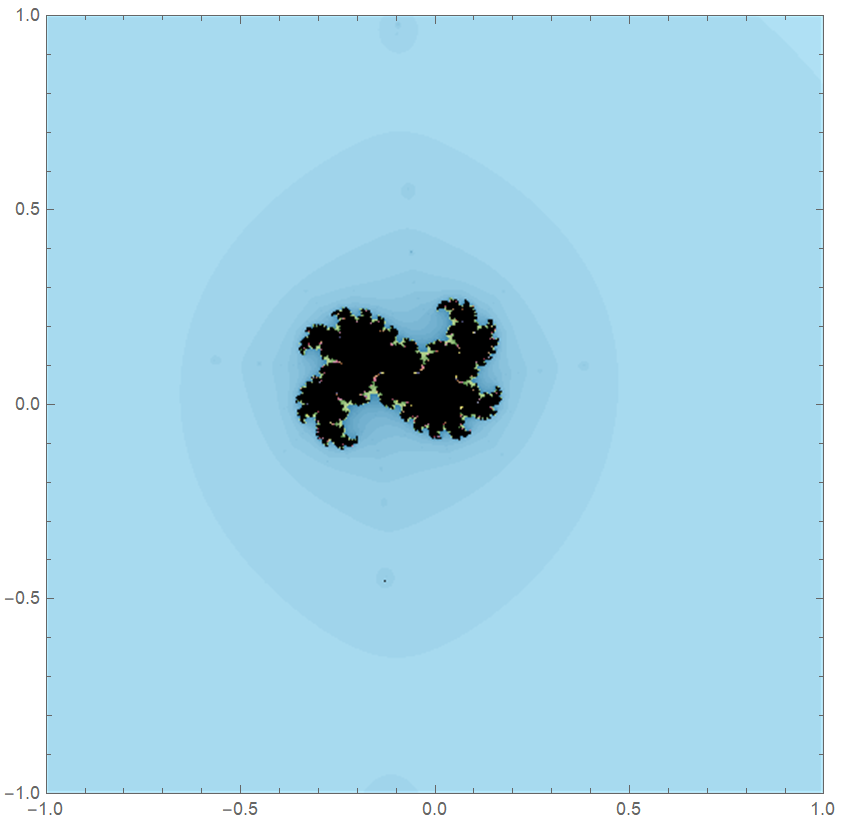
\includegraphics[width=0.4\textwidth,height=0.3\textwidth]{4.PNG}
\caption{Julia set graphs for the polynomial \eqref{eq:polynomial}
when $r=4$, $\theta=\pi$, and $t=0$ (top left), $t=\pi/6$ (top right), 
$t=\pi/3$ (bottom left), $t=\pi/2$ (bottom right).
}
\end{figure}

The rotational symmetry observed in Figure \ref{fig:rotational-symmetry} 
appears to hold for a variety of values of $\theta$ (e.g., square roots of prime numbers, powers of $\pi$, powers of $e$) and most \emph{large} values of $r$ (say, $r>3$),
but seems to fail for most values of $r$ that are closer to $1$. For example, 
Figure \ref{fig:rotational-symmetry-fail} shows the Julia set graphs
when $r=1.612$, $\theta=e^\Phi$ (where $\Phi=(\sqrt{5}+1)/2$ 
is the Golden Ratio), and $t=\pm 1.196$. The two graphs are clearly not
rotations of each other. 
\begin{figure}[H]
\label{fig:rotational-symmetry-fail}
\centering
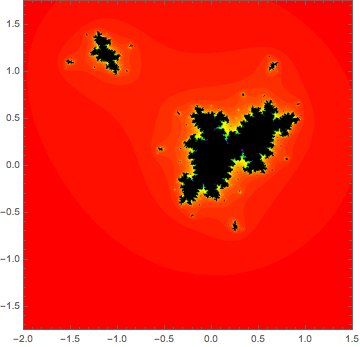
\includegraphics[width=0.4\textwidth]{pi2pi1.png}
\hspace{1em}
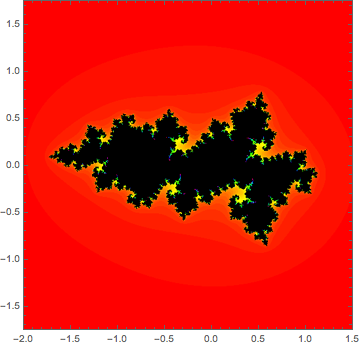
\includegraphics[width=0.4\textwidth]{pi2pi2.png}
\caption{Julia set graphs for the polynomial \eqref{eq:polynomial}
when $r=1.612$, $\theta=e^\Phi$, and $t=-1.196$ (left), $t=1.196$ (right).
}
\end{figure}




\section{Sum-of-Digit Fractals}

Given an integer $b\ge 2$, let  $s_{b}(n)$ denote the sum of the digits
of a number $n$ in base $b$.  For example, in base $b=10$ we have
$s_{10}(15) = 1 + 5 = 6$, while in base $b=2$, $s_{2}(15) =  1 + 1 + 1+
1 = 4$ since $15$ has base $2$ representation $1111$.


\begin{defn}
The \textbf{sum-of-digit fractal} $S(b,p,q)$ for base $b$
and parameters $p$ and $q$ is the graph with steps given by 
\begin{equation}
\label{eq:steps}
e ^ {2 \pi i (s_b(n)/p + n/q)},
\quad n=1,2,3,\dots. 
\end{equation}
\end{defn}
Observe that the steps \eqref{eq:steps} are steps of unit length in 
direction given by the angle $2 \pi  (s_b(n)/p + n/q)$.


In the special case when $q=1$, $p$ is a positive integer, and $b$ is
congruent to $0$ or $1$ modulo $p$, the graphs $S(b,p,q)$
turn out to be finite and can be described precisely as follows:

\begin{thm}[Lehmer \& Lehmer \cite{lehmer-lehmer1979}]
\mbox{}
\begin{itemize}
\item If $b \equiv 1 \pmod{p}$, and $q = 1$, the graph $S(b,p,1)$ 
is a regular $p$-gon.
\item If $b \equiv 0 \pmod{p}$, and $q = 1$, the graph $S(b,p,1)$ 
consists of $p$ rotations of a regular $p$-gon about its center.
\end{itemize}
\end{thm}

In the case where $p$ and $q$ are both integers, but do not satisfy the
conditions of this theorem, the graph $S(b,p,q)$ is in general infinite,
but does exhibit a fractal-like behavior, as illustrated in  Figure
\ref{fig:sum-of-digit-fractal-integer-case}.
\begin{figure}[H]
\label{fig:sum-of-digit-fractal-integer-case}
\centering
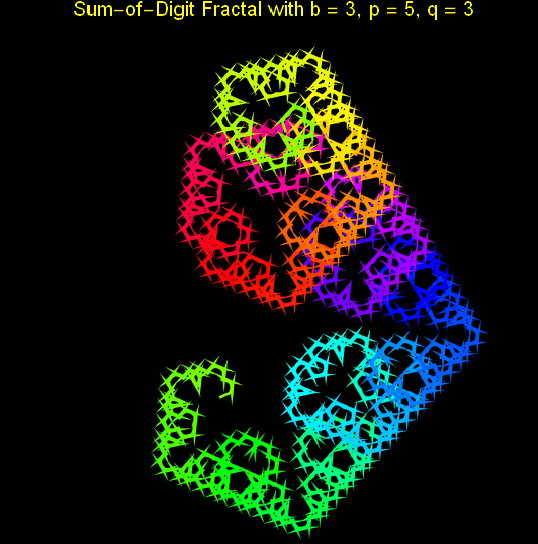
\includegraphics[width=0.4\textwidth]
{n3000v2.png}
\hspace{1em}
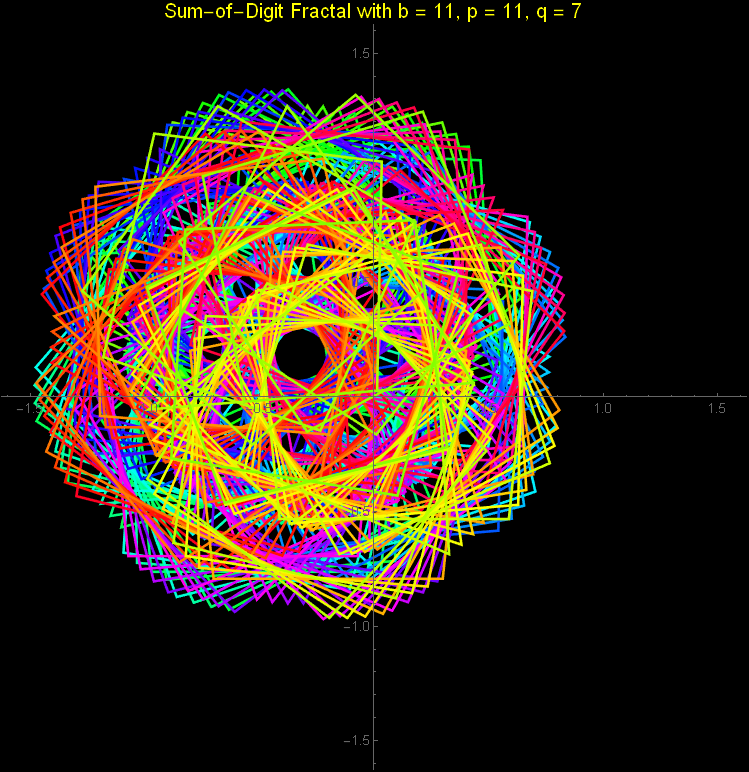
\includegraphics[width=0.4\textwidth]
{n(1000)_b(11)_p(11)_q(7).png}
\caption{Examples of sum-of-digit fractals $S(b,p,q)$ with 
integer parameters $p$ and $q$. The left figure shows the 
first $3000$ steps of $S(3,5,3)$. 
The right figure shows the 
first $1000$ steps of $S(11,11,7)$. 
}
\end{figure}

The most interesting case is the case where at least one of $p$ and $q$
is irrational.  In this case, the graph $S(b,p,q)$ can take on a
remarkable variety of shapes, from fractal-like features to distinctive
geometric patterns to random clouds, as illustrated in  Figure
\ref{fig:sum-of-digit-fractal-irrational-case}.  See Dekking
\cite{dekking1982} and Dekking \& Mend\'es-France
\cite{dekking-mendes-france1981} for further examples and some theoretical results. 

\begin{figure}[H]
\label{fig:sum-of-digit-fractal-irrational-case}
\centering
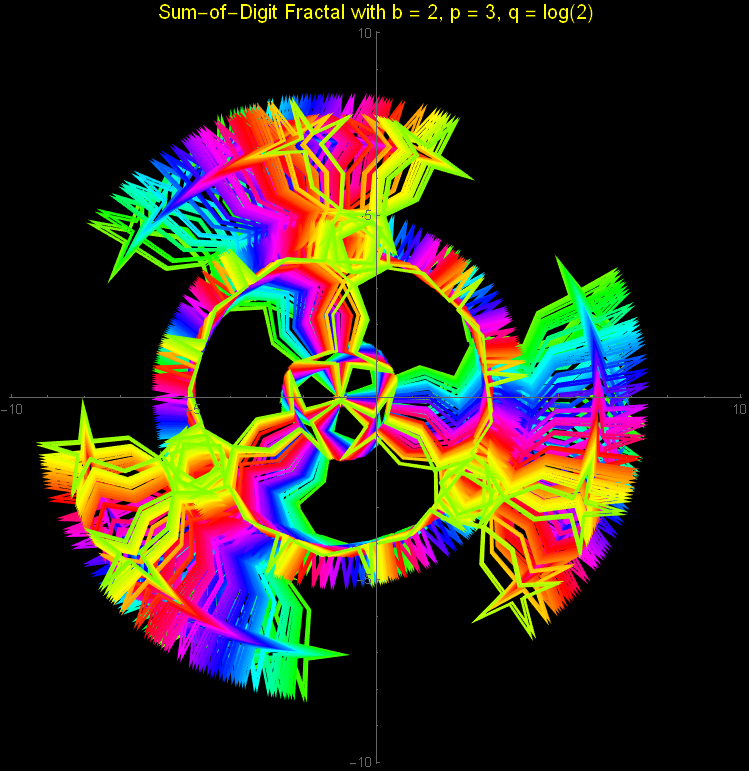
\includegraphics[width=0.4\textwidth]
{n(10000)_b(2)_p(3)_q(ln2).png}
\hspace{1em}
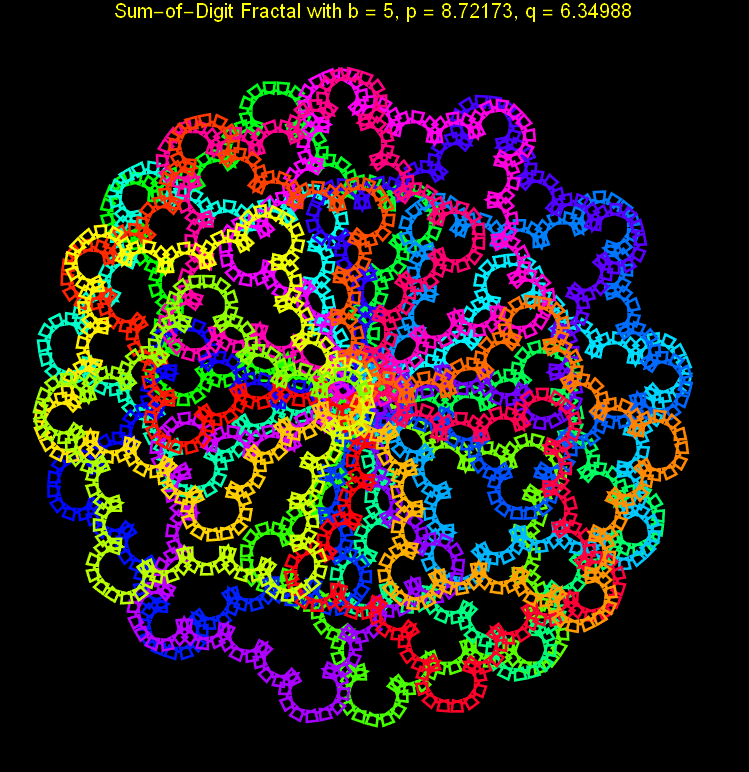
\includegraphics[width=0.4\textwidth]
{n(10000)_b(5)_p(8dot72)_q(6dot34).png}
\caption{Examples of sum-of-digit fractals $S(b,p,q)$ with 
irrational parameters. The left figure shows the 
first $10000$ steps of $S(2,3,\ln 2)$. 
The right figure shows the 
first $10000$ steps of $S(5,8.72,6.34)$. 
}
\end{figure}


\begin{thebibliography}{99}

\bibitem{beardon}
A.F. Beardon,
``Iteration of Rational Functions: Complex Analytic Dynamical Systems'',
\textit{Springer}, 1991.

\bibitem{carleson-gamelin}
L. Carleson and T.W. Gamelin, ``Complex Dynamics'',
\textit{Springer}, 1993.


\bibitem{dekking1982}
F.M. Dekking, ``On the distribution of digits in arithmetic sequences'',
\textit{Séminaire de théorie des nombres de Bordeaux}, 1--12 (1981).

\bibitem{dekking-mendes-france1981}
F.M. Dekking and M. Mend\`es France, M, 
``Uniform distribution modulo one: a geometrical viewpoint'', 
\textit{Journal f\"ur die reine und angewandte Mathematik} \textbf{329}
(1981),  143--153.
\bibitem{lehmer-lehmer1979} 
D.H. Lehmer and E. Lehmer,  ``Picturesque exponential sums, I'',
\textit{The American Mathematical Monthly} \textbf{86} (1979), 725--733.

\bibitem{WD}
Wolfram Demonstrations Project, \url{https://demonstrations.wolfram.com}.

\end{thebibliography}


\end{document}
